\documentclass[12pt]{article}
\usepackage[utf8]{inputenc} % nastavuje pou�it� k�dov�n�, u�ivatel� Windows zam�n� latin2 za cp1250
\usepackage[T1]{fontenc}
\usepackage{a4wide} % nastavuje standardn� evropsk� form�t str�nek A4
%\usepackage{index} % nutno pou��t v p��pad� tvorby rejst��ku bal��kem makeindex
%\usepackage{fancybox} % umo��uje pokro�il� r�me�kov�n� :-)
\usepackage{graphicx} % nezbytn� pro standardn� vkl�d�n� obr�zk� do dokumentu
\usepackage{enumerate}
\usepackage{listings}
\usepackage[dvips]{color}
\usepackage{subfigure}
\usepackage{amssymb,amsmath}

\setlength{\parindent}{0pt} 
\setlength{\parskip}{2ex}

\title{Solution for assignment \#1}
\date{October 27, 2012}
\author{Vojtech Kopal}

\newcommand{\mytilde}{\raise.17ex\hbox{$\scriptstyle\mathtt{\sim}$} }

\begin{document}

\maketitle

\clearpage

\section{Economic part}

\subsection*{a) Economic growth and convergence - descriptive statistics:}

\begin{figure}[h!]
  \centering           
  \subfigure{                         
  	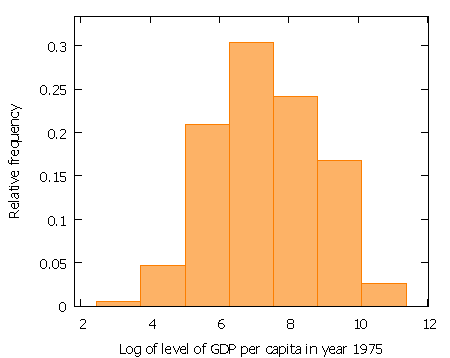
\includegraphics{graphs/1a/gdp1975.pdf}
  	\label{1a:gpd1975}
  }                   
  \subfigure{                         
  	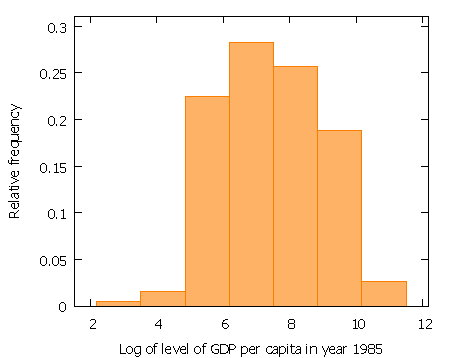
\includegraphics{graphs/1a/gdp1985.pdf}
  	\label{1a:gpd1985}
  }                 
  \subfigure{                         
  	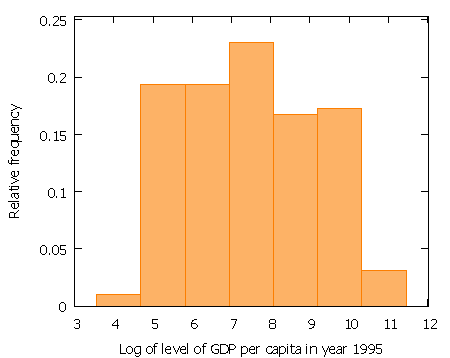
\includegraphics{graphs/1a/gdp1995.pdf}
  	\label{1a:gpd1995}
  }                 
  \subfigure{                         
  	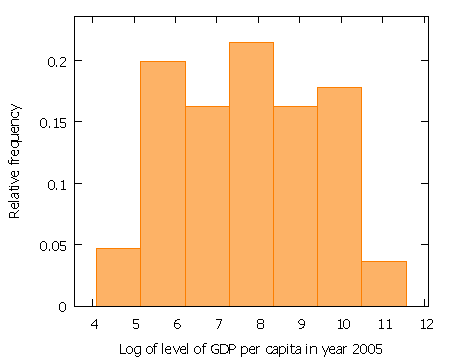
\includegraphics{graphs/1a/gdp2005.pdf}
  	\label{1a:gpd2005}
  }                         
  \caption{Bla.}
\end{figure}

\end{document}